\section{Parity Robustness}
\label{sec:results-parity}

Figure~\ref{fig:parity-robustness} is the empirical anchor for the title claim of the paper. The parity-sector laboratory is designed around controlled leakage between the even- and odd-parity sectors of a two-bit system, so the natural candidate coarse variable is the parity bit \(a \oplus b\). We compare that lens against two alternatives defined on the same underlying four macrostates: the familiar Boolean predicate \(a \wedge b\), and the median of a family of balanced random binary partitions. The comparison is intentionally closure-based rather than purely predictive. The plotted quantity is route mismatch (RM), so smaller values mean that the proposed binary variable is better aligned with the induced coarse dynamics.

\begin{figure}[t]
    \centering
    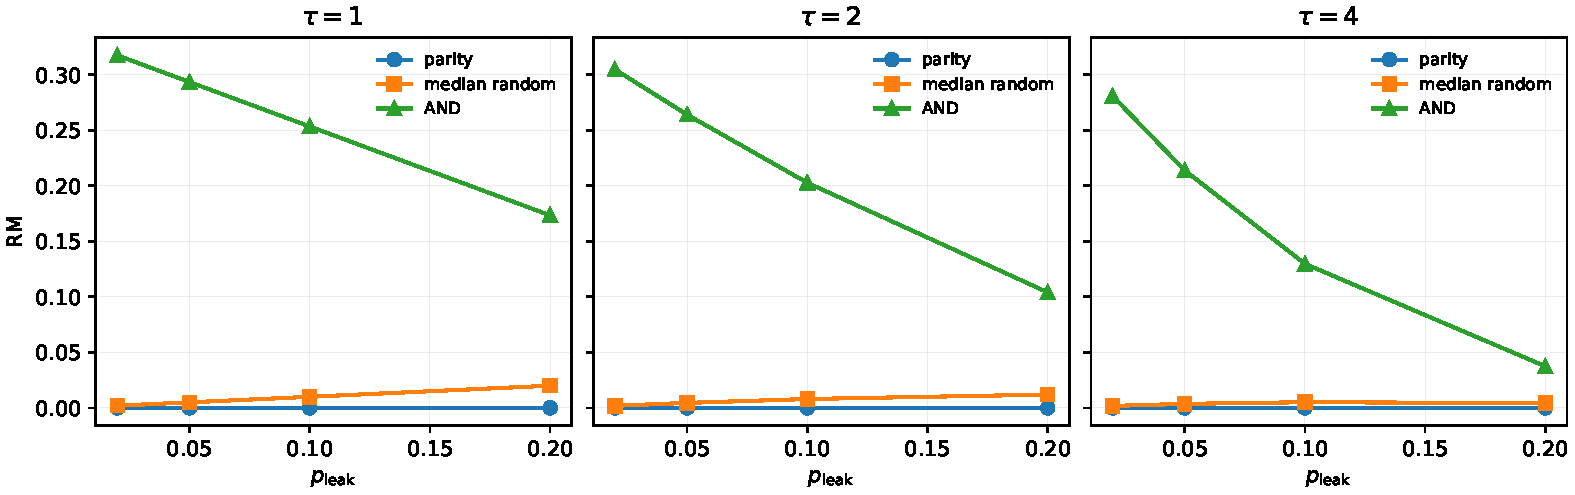
\includegraphics[width=\linewidth]{figures/parity_robustness.pdf}
    \caption{Route mismatch in the parity-sector laboratory for three candidate binary coarse variables: the parity lens \(a \oplus b\), the AND lens \(a \wedge b\), and the median balanced random binary partition. Each panel fixes \(\tau\) and scans leakage \(p_{\mathrm{leak}}\). Across the full tested grid, the parity lens remains essentially closure-aligned while the AND and median-random alternatives show systematically larger mismatch. The figure is rendered directly from \protect\path{results/final_claims/figure_parity_robustness.csv}.}
    \label{fig:parity-robustness}
\end{figure}

The main result is absolute across the tested grid. In the frozen bundle, the parity lens beats the median random binary partition at every one of the \(12\) \((p_{\mathrm{leak}},\tau)\) grid points, giving a win rate of \(1\). The representative values recorded in the claim ledger make the point sharply. At \(p_{\mathrm{leak}}=0.05\) and \(\tau=1\), the parity RM is \(1.11\times 10^{-16}\), whereas the median random RM is \(0.005\). At \(p_{\mathrm{leak}}=0.20\) and \(\tau=1\), the parity RM is \(0\), whereas the median random RM is \(0.020\). On the same two slices, the AND lens is far less closure-aligned, with RM \(0.293\) at \(p_{\mathrm{leak}}=0.05,\tau=1\) and RM \(0.173\) at \(p_{\mathrm{leak}}=0.20,\tau=1\). Figure~\ref{fig:parity-robustness} shows that this is not an isolated comparison point but the qualitative pattern across all three timescales.

What makes the result conceptually useful is that parity remains closure-aligned even when it becomes noisy as a signal. The parity error grows from \(0.05\) at \(p_{\mathrm{leak}}=0.05,\tau=1\) to \(0.20\) at \(p_{\mathrm{leak}}=0.20,\tau=1\), and at longer horizons it grows further, reaching \(0.4352\) at \(p_{\mathrm{leak}}=0.20,\tau=4\). Stability degrades in the same direction, from \(0.95\) at \(p_{\mathrm{leak}}=0.05,\tau=1\) to \(0.5648\) at \(p_{\mathrm{leak}}=0.20,\tau=4\). Yet the parity RM remains numerically near zero throughout the grid. This is exactly the distinction the framework is designed to expose. A coarse variable can become less predictable under leakage and still remain the correct closure variable for the layer. Robustness here does not mean error-free transmission; it means that the packaged distinction continues to define the right macro partition for the induced dynamics.

The contrast with AND makes the structural point. AND is not a random or adversarial choice: it is a perfectly familiar Boolean predicate on the same underlying bits. But in the parity-sector laboratory it cuts across the dominant sector structure rather than aligning with it. Its RM remains orders of magnitude above the parity RM across the grid, and above the median random partition at every reported point. The lesson is that semantically familiar predicates are not automatically closure-friendly. A substrate does not inherit its logic from our preferred vocabulary; it selects the distinctions that its own dynamics can stabilize.

This is why XOR appears in the title. In the present laboratory, parity is the earliest and cleanest packaged invariant: it compresses the microstate space in the same way the dynamics itself organizes it. The more modest point is that variables aligned with a laboratory's dominant invariant or sector structure can be especially natural closure variables \cite{simonando1961aggregation,shalizi2025macrostate,barnettseth2023dynamical}. The next section asks how far that observation extends once we move from a single robust coarse variable to full gate families under noise, staging, and timescale stress (Section~\ref{sec:results-phase}).
